\chapter{Motivation}\label{sec:einleitung}

  Das Wort Plasma (altgriechisch $\uppi\uplambda\upalpha\upsigma\upmu\upalpha$) steht für ein Gebilde, welches aus verschiedenen Komponenten zusammengesetzt ist und eine kollektive, "`lebendige"' Dynamik besitzt. Ebenso wie in einer Suspension verändern kolloidale Teilchen in Plasmen die Eigenschaften dieses Kollektivismus. Viele Phänomene wie Wellen oder besondere Ladungsträger-Wechselwirkungen in Gasentladungen können, mit Hilfe der Physik \tilt{kolloidaler (komplexer) Plasmen} besser verstanden und untersucht werden. Zudem entdeckt man, durch das Einbringen makroskopischer Festkörper in die Entladung, zusätzlich neue Effekte innerhalb dieser staubigen Plasmen. Die Beschreibung von Gasen im sog. \tilt{vierten Aggregatzustand} mit der Magnetohydrodynamik erleichtert insbesondere das theoretische Verständnis der Dynamik der aufgeladenen Partikel. Angelehnt an dieses Prinzip ist auch die Interpretation der, in diesem Experiment erzeugten \tilt{finiten Yukawa-Cluster} - u.a. auf Grund elektrostatischer Wechselwirkungen levitierende Gruppen von bis zu 50 Staub-Partikel - als "`Tropfen"' vor dem Hintergrund des Plasmas.\\
  Das Feld der Physik komplexer Plasmen vergrößert sich rasant: nicht nur im Labor, sonder auch bei Experimenten in Schwerelosigkeit oder für Optimierungen der Elektronik-Industrie sind staubige Gasentladungen von großem Interesse. Im Speziellen sind komplexer Plasmen in der Astrophysik sehr wichtig, da sich 99\% des beobachtbaren Volumens im Weltall im Plasma-Zustand befindet. Interstellare Gaswolken, Kometen-Schweife und planetare Ringe wie um Saturn sind alles staubige Plasmen.\\
  Ziel dieser Arbeit soll die präzise Manipulation eines solchen finiten Yukawa-Systems sein. Es soll der Zusammenhang zwischen unterschiedlichen Moden-Theorien zur kollektiven Beschreibung eines Clusters hergestellt werden. Die Frage die sich den Versuchen dieser Arbeit zu Grunde legt, beschäftigt sich demnach mit der Verbindung der Fluid-Theorie und dem Eigenwertproblem eines Yukawa-Balls. Dafür wird zudem die Anregung durch segmentierte Kupferringe über den Vergleich der Ergebnisse mit erfolgreichen Manipulationen von Normalmoden (aus \cite{Mulsow13}) gerechtfertigt. Dafür wichtige Bedingungen der lokalen Entladung um den eingefangenen "`Ball"' wurden ebenfalls untersucht. Von besonderem Gewicht war dabei die Methodik der Stereoskopie und des elektrischen Einfangs. Bei ersterem handelt es sich um die dreidimensionale Rekonstruktion aus zweidimensionalen Informationen verschiedener Kamera-Blickwinkel. Letzteres beschreibt die Art und Weise, wie die Manipulation der Cluster vorgenommen wurde. Hierfür wurden eigens verschiedenen, segmentierte Ring-Elektroden aus Kupfer für die Experimente dieser Arbeit konzipiert und konstruiert.\newline

  \begin{figure}[!h]
  \centering
    \begin{minipage}{0.49\textwidth}
      \centering
      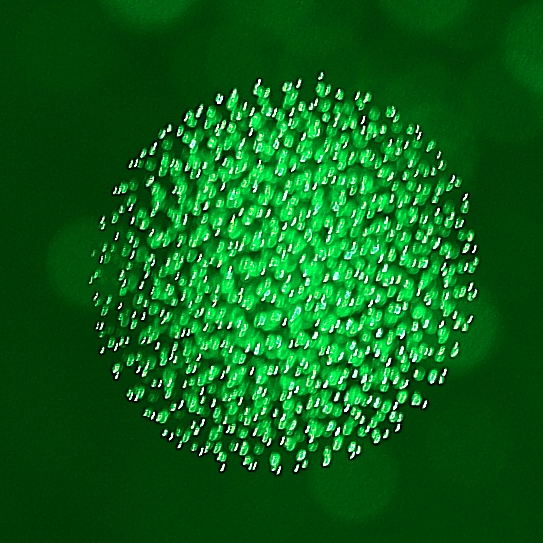
\includegraphics[scale=1.]{figs/cluster.png}
    \end{minipage}
    \begin{minipage}{0.48\textwidth}
      \caption{Mit grünen Nd:YAG-Lasern ausgeleuchteter Yukawa-Ball. Der verwendete Staub  betsteht aus homogenen, Malamin-Formaldehyd-Kügelchen mit einem Radius im $\upmu$m-Bereich}
    \end{minipage}
  \end{figure}
